\documentclass{standalone}
\usepackage{tikz}
\usetikzlibrary{patterns, positioning}

\begin{document}
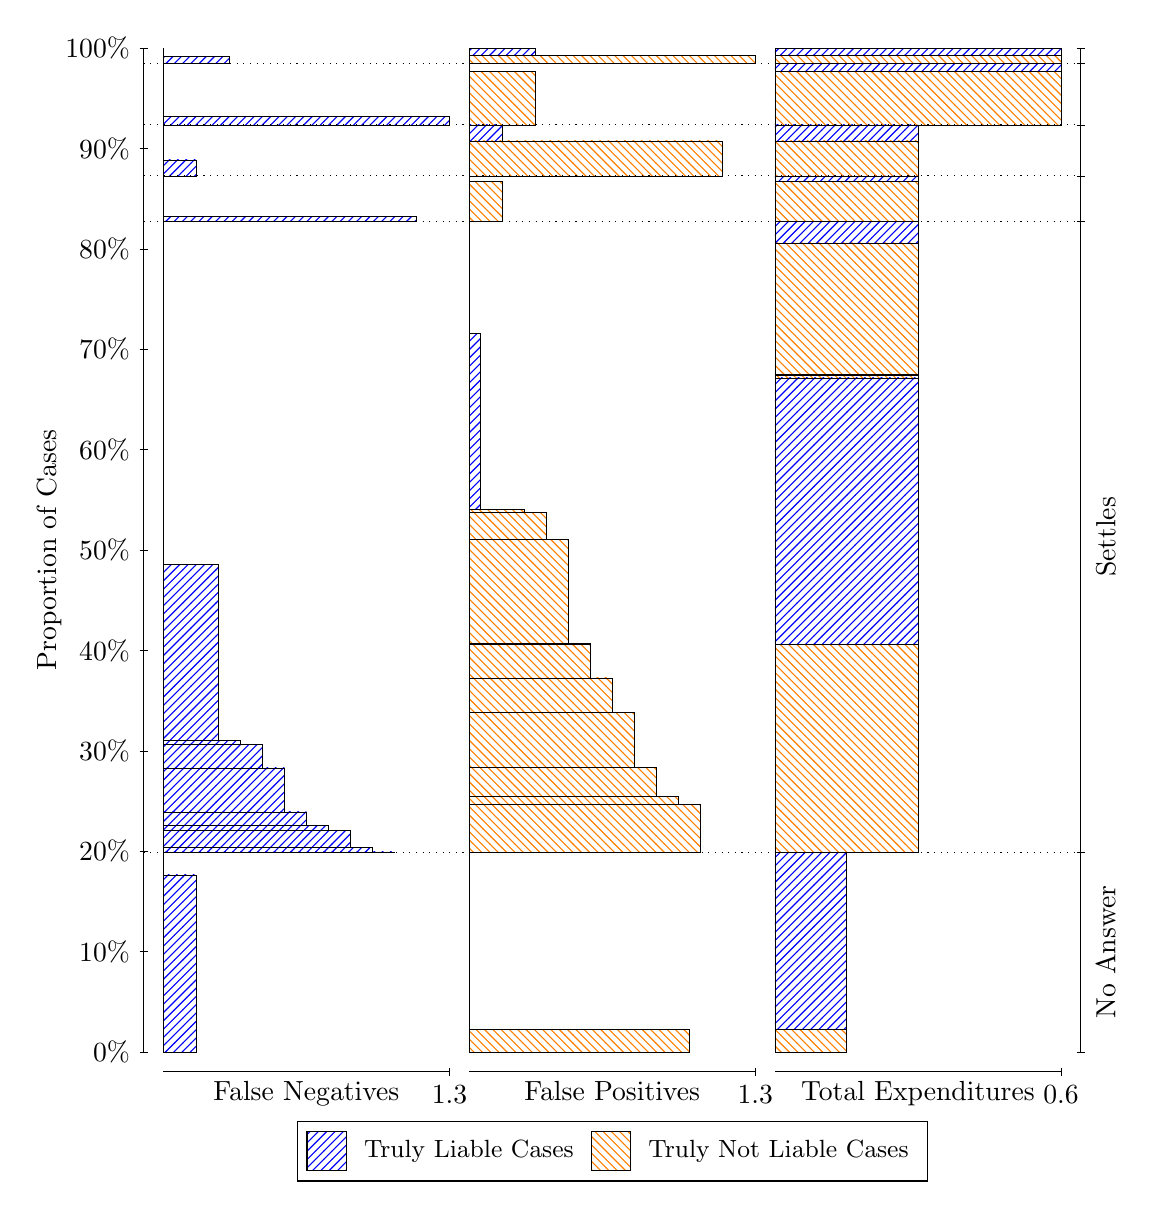
\begin{tikzpicture}
\draw[black, very thin] (1.5,1.75) -- (1.5,14.5);
\node[rotate=90, anchor=center] at (0.3, 8.125) {Proportion of Cases};
\draw[black, very thin] (1.45,1.75) -- (1.55,1.75);
\node[anchor=east] at (1.45, 1.75) {0\%};
\draw[black, very thin] (1.45,3.025) -- (1.55,3.025);
\node[anchor=east] at (1.45, 3.025) {10\%};
\draw[black, very thin] (1.45,4.3) -- (1.55,4.3);
\node[anchor=east] at (1.45, 4.3) {20\%};
\draw[black, very thin] (1.45,5.575) -- (1.55,5.575);
\node[anchor=east] at (1.45, 5.575) {30\%};
\draw[black, very thin] (1.45,6.85) -- (1.55,6.85);
\node[anchor=east] at (1.45, 6.85) {40\%};
\draw[black, very thin] (1.45,8.125) -- (1.55,8.125);
\node[anchor=east] at (1.45, 8.125) {50\%};
\draw[black, very thin] (1.45,9.4) -- (1.55,9.4);
\node[anchor=east] at (1.45, 9.4) {60\%};
\draw[black, very thin] (1.45,10.675) -- (1.55,10.675);
\node[anchor=east] at (1.45, 10.675) {70\%};
\draw[black, very thin] (1.45,11.95) -- (1.55,11.95);
\node[anchor=east] at (1.45, 11.95) {80\%};
\draw[black, very thin] (1.45,13.225) -- (1.55,13.225);
\node[anchor=east] at (1.45, 13.225) {90\%};
\draw[black, very thin] (1.45,14.5) -- (1.55,14.5);
\node[anchor=east] at (1.45, 14.5) {100\%};

\draw[black, very thin] (13.4,1.75) -- (13.4,14.5);
\draw[black, very thin] (13.35,1.75) -- (13.45,1.75);
\node[anchor=west] at (13.35, 1.75) {};
\draw[black, very thin] (13.35,4.2865) -- (13.45,4.2865);
\node[anchor=west] at (13.35, 4.2865) {};
\draw[black, very thin] (13.35,12.296) -- (13.45,12.296);
\node[anchor=west] at (13.35, 12.296) {};
\draw[black, very thin] (13.35,12.876) -- (13.45,12.876);
\node[anchor=west] at (13.35, 12.876) {};
\draw[black, very thin] (13.35,13.525) -- (13.45,13.525);
\node[anchor=west] at (13.35, 13.525) {};
\draw[black, very thin] (13.35,14.305) -- (13.45,14.305);
\node[anchor=west] at (13.35, 14.305) {};
\draw[black, very thin] (13.35,14.5) -- (13.45,14.5);
\node[anchor=west] at (13.35, 14.5) {};

\draw[black, very thin, pattern color=blue, pattern=north east lines] (1.75,1.75) rectangle (2.1692,3.999);
\draw[black, very thin, pattern color=orange, pattern=north west lines] (1.75,3.999) rectangle (1.75,4.2865);
\draw[black, very thin, pattern color=blue, pattern=north east lines] (1.75,4.2865) rectangle (4.6846,4.2919);
\draw[black, very thin, pattern color=blue, pattern=north east lines] (1.75,4.2919) rectangle (4.4051,4.3438);
\draw[black, very thin, pattern color=blue, pattern=north east lines] (1.75,4.3438) rectangle (4.1256,4.5604);
\draw[black, very thin, pattern color=blue, pattern=north east lines] (1.75,4.5604) rectangle (3.8462,4.6283);
\draw[black, very thin, pattern color=blue, pattern=north east lines] (1.75,4.6283) rectangle (3.5667,4.7988);
\draw[black, very thin, pattern color=blue, pattern=north east lines] (1.75,4.7988) rectangle (3.2872,5.3568);
\draw[black, very thin, pattern color=blue, pattern=north east lines] (1.75,5.3568) rectangle (3.0077,5.6518);
\draw[black, very thin, pattern color=blue, pattern=north east lines] (1.75,5.6518) rectangle (2.7282,5.706);
\draw[black, very thin, pattern color=blue, pattern=north east lines] (1.75,5.706) rectangle (2.4487,7.9436);
\draw[black, very thin, pattern color=orange, pattern=north west lines] (1.75,7.9436) rectangle (1.75,12.296);
\draw[black, very thin, pattern color=blue, pattern=north east lines] (1.75,12.296) rectangle (4.9641,12.362);
\draw[black, very thin, pattern color=orange, pattern=north west lines] (1.75,12.362) rectangle (1.75,12.876);
\draw[black, very thin, pattern color=blue, pattern=north east lines] (1.75,12.876) rectangle (2.1692,13.08);
\draw[black, very thin, pattern color=orange, pattern=north west lines] (1.75,13.08) rectangle (1.75,13.525);
\draw[black, very thin, pattern color=blue, pattern=north east lines] (1.75,13.525) rectangle (5.3833,13.631);
\draw[black, very thin, pattern color=orange, pattern=north west lines] (1.75,13.631) rectangle (1.75,14.305);
\draw[black, very thin, pattern color=blue, pattern=north east lines] (1.75,14.305) rectangle (2.5885,14.397);
\draw[black, very thin, pattern color=orange, pattern=north west lines] (1.75,14.397) rectangle (1.75,14.5);
\draw[black, very thin, pattern color=orange, pattern=north west lines] (5.6333,1.75) rectangle (8.4282,2.0375);
\draw[black, very thin, pattern color=blue, pattern=north east lines] (5.6333,2.0375) rectangle (5.6333,4.2865);
\draw[black, very thin, pattern color=orange, pattern=north west lines] (5.6333,4.2865) rectangle (8.5679,4.8975);
\draw[black, very thin, pattern color=orange, pattern=north west lines] (5.6333,4.8975) rectangle (8.2885,4.9912);
\draw[black, very thin, pattern color=orange, pattern=north west lines] (5.6333,4.9912) rectangle (8.009,5.3664);
\draw[black, very thin, pattern color=orange, pattern=north west lines] (5.6333,5.3664) rectangle (7.7295,6.0664);
\draw[black, very thin, pattern color=orange, pattern=north west lines] (5.6333,6.0664) rectangle (7.45,6.5019);
\draw[black, very thin, pattern color=orange, pattern=north west lines] (5.6333,6.5019) rectangle (7.1705,6.9286);
\draw[black, very thin, pattern color=orange, pattern=north west lines] (5.6333,6.9286) rectangle (7.1705,6.9358);
\draw[black, very thin, pattern color=orange, pattern=north west lines] (5.6333,6.9358) rectangle (6.891,8.2601);
\draw[black, very thin, pattern color=orange, pattern=north west lines] (5.6333,8.2601) rectangle (6.6115,8.6002);
\draw[black, very thin, pattern color=orange, pattern=north west lines] (5.6333,8.6002) rectangle (6.3321,8.6386);
\draw[black, very thin, pattern color=blue, pattern=north east lines] (5.6333,8.6386) rectangle (5.7731,10.876);
\draw[black, very thin, pattern color=blue, pattern=north east lines] (5.6333,10.876) rectangle (5.6333,12.296);
\draw[black, very thin, pattern color=orange, pattern=north west lines] (5.6333,12.296) rectangle (6.0526,12.809);
\draw[black, very thin, pattern color=blue, pattern=north east lines] (5.6333,12.809) rectangle (5.6333,12.876);
\draw[black, very thin, pattern color=orange, pattern=north west lines] (5.6333,12.876) rectangle (8.8474,13.321);
\draw[black, very thin, pattern color=blue, pattern=north east lines] (5.6333,13.321) rectangle (6.0526,13.525);
\draw[black, very thin, pattern color=orange, pattern=north west lines] (5.6333,13.525) rectangle (6.4718,14.199);
\draw[black, very thin, pattern color=blue, pattern=north east lines] (5.6333,14.199) rectangle (5.6333,14.305);
\draw[black, very thin, pattern color=orange, pattern=north west lines] (5.6333,14.305) rectangle (9.2667,14.408);
\draw[black, very thin, pattern color=blue, pattern=north east lines] (5.6333,14.408) rectangle (6.4718,14.5);
\draw[black, very thin, pattern color=orange, pattern=north west lines] (9.5167,1.75) rectangle (10.425,2.0375);
\draw[black, very thin, pattern color=blue, pattern=north east lines] (9.5167,2.0375) rectangle (10.425,4.2865);
\draw[black, very thin, pattern color=orange, pattern=north west lines] (9.5167,4.2865) rectangle (11.333,6.9286);
\draw[black, very thin, pattern color=blue, pattern=north east lines] (9.5167,6.9286) rectangle (11.333,10.31);
\draw[black, very thin, pattern color=orange, pattern=north west lines] (9.5167,10.31) rectangle (11.333,10.349);
\draw[black, very thin, pattern color=blue, pattern=north east lines] (9.5167,10.349) rectangle (11.333,10.354);
\draw[black, very thin, pattern color=orange, pattern=north west lines] (9.5167,10.354) rectangle (11.333,12.026);
\draw[black, very thin, pattern color=blue, pattern=north east lines] (9.5167,12.026) rectangle (11.333,12.296);
\draw[black, very thin, pattern color=orange, pattern=north west lines] (9.5167,12.296) rectangle (11.333,12.809);
\draw[black, very thin, pattern color=blue, pattern=north east lines] (9.5167,12.809) rectangle (11.333,12.876);
\draw[black, very thin, pattern color=orange, pattern=north west lines] (9.5167,12.876) rectangle (11.333,13.321);
\draw[black, very thin, pattern color=blue, pattern=north east lines] (9.5167,13.321) rectangle (11.333,13.525);
\draw[black, very thin, pattern color=orange, pattern=north west lines] (9.5167,13.525) rectangle (13.15,14.199);
\draw[black, very thin, pattern color=blue, pattern=north east lines] (9.5167,14.199) rectangle (13.15,14.305);
\draw[black, very thin, pattern color=orange, pattern=north west lines] (9.5167,14.305) rectangle (13.15,14.408);
\draw[black, very thin, pattern color=blue, pattern=north east lines] (9.5167,14.408) rectangle (13.15,14.5);
\draw[black, dotted] (1.5,4.2865) -- (13.4,4.2865);
\draw[black, dotted] (1.5,12.296) -- (13.4,12.296);
\draw[black, dotted] (1.5,12.876) -- (13.4,12.876);
\draw[black, dotted] (1.5,13.525) -- (13.4,13.525);
\draw[black, dotted] (1.5,14.305) -- (13.4,14.305);
\draw[black, very thin] (1.75,1.5) -- (5.3833,1.5);
\node[anchor=north] at (3.5667, 1.5) {False Negatives};
\draw[black, very thin] (5.3833,1.45) -- (5.3833,1.55);
\node[anchor=north] at (5.3833, 1.45) {1.3};

\draw[black, very thin] (5.6333,1.5) -- (9.2667,1.5);
\node[anchor=north] at (7.45, 1.5) {False Positives};
\draw[black, very thin] (9.2667,1.45) -- (9.2667,1.55);
\node[anchor=north] at (9.2667, 1.45) {1.3};

\draw[black, very thin] (9.5167,1.5) -- (13.15,1.5);
\node[anchor=north] at (11.333, 1.5) {Total Expenditures};
\draw[black, very thin] (13.15,1.45) -- (13.15,1.55);
\node[anchor=north] at (13.15, 1.45) {0.6};

\node[black, centered, rotate=90] at (13.72, 3.0182) {No Answer};
\node[black, centered, rotate=90] at (13.72, 8.2911) {Settles};





\draw (7.449999999999999,1.5) node[draw=none] (baseCoordinate) {};
\begin{scope}[align=center]
        \matrix[scale=0.5, draw=black, below=0.5cm of baseCoordinate, nodes={draw}, column sep=0.1cm]{
            \node[rectangle, draw, minimum width=0.5cm, minimum height=0.5cm, pattern=north east lines, pattern color=blue] {}; &
            \node[draw=none, font=\small] (B) {Truly Liable Cases}; &
            \node[rectangle, draw, minimum width=0.5cm, minimum height=0.5cm, pattern=north west lines, pattern color=orange] {}; &
            \node[draw=none, font=\small] (B) {Truly Not Liable Cases}; \\
            };
\end{scope}

\end{tikzpicture}
\end{document}